\section{Programmerings opgaver}



\subsection*{Programmering opgaver 1.}



\subsection*{Programmering opgaver 2.}



\subsection*{Programmering opgaver 3.}


\subsection*{Tids overvejelser}
\subsubsection*{Hvordan beregnes tiden af en funktion i Python}
For at få konkrete værdier for hvor lang tid det tager metoderne at beregne PageRank værdierne, så brugte vi \emph{time} modulet indbygget i Python. Her kan der bruges \texttt{time.time()} til at gemme en start-tid før funktionen er startet og en tid når den er stoppet. Den totale tid det tager beregnes så ved at trække start-tiden fra stop-tiden.

\subsubsection*{Analyse af data}
\begin{table}[!h]
    \centering
    \begin{tabular}{c|l|l|l|l}
        \# hjemmesider & Random Surfer & Recursive & Limit & Eigenvectors \\
        \hline
        $N = 10$       & 1.8134 s   & 0.0000 s   & 0.0000 s   & 0.0010 s   \\
        $N = 75$       & 3.4769 s   & 0.0110 s   & 0.0020 s   & 0.0028 s   \\
        $N = 250$      & 7.6943 s   & 0.0860 s   & 0.0090 s   & 0.0699 s
    \end{tabular}
    \caption{En tabel over metodernes tidsforbrug afhængigt at $n$, antallet af webpages i simulationen. Når der står "0.0000" så betyder det ikke faktisk 0, men skyldes numeriske fejl fra python fordi tallet er så lille. Her refererer "Random Surfer" til Random surfer modellen med en dæmpningsfaktor, "Recursive" er den rekursive model, "Limit" er hvor der anvendes at $A$ er en \textit{Markov matrix} med positive værdier og "Eigenvectors er hvor der findes den korrekte egenvektor og den skaleres tilpasseligt. Naturligvis er dæmpningsfaktoren $d$ ens for alle modellerne som er $d = 0.85$.}
    \label{tidsFigur}
\end{table}

\begin{figure}
    \centering
    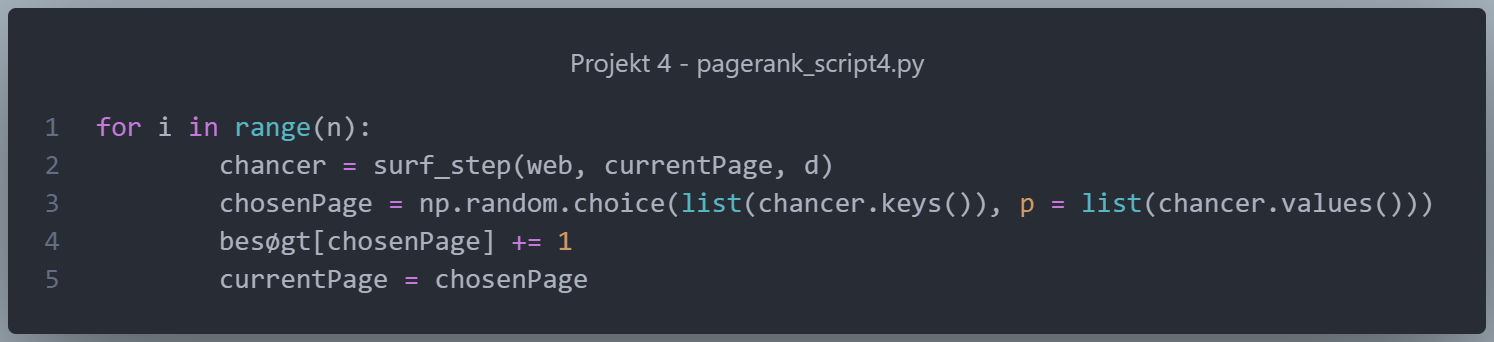
\includegraphics[width = \linewidth]{Kode1.png}
    \caption{Del af kode fra \texttt{random\_surfer} funktionen}
\end{figure}


På Tabel~\ref{tidsFigur}, kan det ses at Random Surfer modellen er den klart mest langsomme model som der er. Dette giver også mening siden at der for hver iteration af algoritmen skal køres \texttt{surf\_step} funktionen, som beregner sandsynlighedsfordelingen. En hurtig måde der kunne skæres ned på tiden brugt i denne funktion, vil være ved at gemme resultatet af \texttt{surf\_step} og så genbruge det, så det ikke skal beregnes hver gang igen.

Det kan ses ved at kigge på alle resultaterne at Limit-metoden er klart den hurtigste. Denne I dette tilfælde har vi dog ganget matricen med sig selv 20 gange. Denne værdi kan forøges så meget som man vil, på bekostningen af det så vil tage længere tid, men resultatet vil blive mere præcist.

Den rekursive model kan også tilpasses så den tager mindre tid, ved at ændre på \texttt{stopvalue} eller \texttt{max\_iterations}.

Egenværdi metoden virker som den som generelt er bedst, da den finder den matematiske korrekte løsning og tager meget kort tid


